\documentclass[notheorems]{beamer} % 必须[notheorems], 否则与自定义的定理环境冲突
\usepackage{wcbeamer}


\title{程序综合\\ 报告}
\author{唐雯豪, 易普, 谢睿峰}
\institute{EECS, PKU}
\date{\today}
\background{15251.pdf}

\AtBeginSection{
  \begin{frame}<beamer>
    \frametitle{Outline}
    \tableofcontents[currentsection]
  \end{frame}
}

\begin{document}
  \maketitle

  \section{概述}
  \begin{frame}
    \frametitle{概述}
    我们小组设计并实现了四种方法,最后提交的程序使用了其中三种方法并行求解,可以解出open tests中所有测试用例,并且具有一定泛化能力。
  \end{frame}
  
  \section{方法一:VSA}
  \begin{frame}
    \frametitle{算法过程}
    和上课讲的基本相同:
    \begin{enumerate}
      \item 随机生成几个样例
      \item 从样例中生成VSA并求交
      \item 从求交后的VSA中生成任意一个程序
      \item 扔给SMT solver,有反例的话从反例生成VSA并跟当前VSA求交,重复上一步;否则得到结果
    \end{enumerate}
  \end{frame}
  \begin{frame}
    \frametitle{效果}
    写得太差了,只能解出three和max2

    max3中随着样例数量增加,VSA中非终结符数量的增长:
    33 $\to$ 208 $\to$ 1466 $\to$  10251 $\to$  71990 $\to$ VSA求交函数爆栈

    沉没成本,果断放弃
  \end{frame}
  \section{方法二:直接法}

  \begin{frame}
    \frametitle{观察}
    \begin{enumerate}
      \item SyGuS问题直接给了我们对函数结果的约束
      \item 大多数对函数结果的约束都是等号约束
      \begin{itemize}
        \item 对于open tests来说,除了max系列问题之外都是只有等号约束
        \item 并且除了three问题之外,所有等号约束都是函数结果只出现在等号一边(也就是没有递归约束)
      \end{itemize}
    \end{enumerate}
    $\to$ \textbf{直接}从约束中综合出程序。
  \end{frame}
  \begin{frame}
    \frametitle{算法过程}
    主要想法:提取每个对函数结果的等号约束成立时的条件,然后把整个程序写成一堆if语句。

    具体分为三个步骤:
    \begin{enumerate}
      \item 约束规范化
      \item 分支提取
      \item 局部搜索
    \end{enumerate}
  \end{frame}
  \begin{frame}
    \frametitle{约束规范化}
    \begin{enumerate}
      \item 将所有constraint语句用and连起来
      \item 对于传递了常数的函数调用,将常数参数作为一个条件前置,比如将 $f\ 3\ ... = y$ 转化成 $(x = 3)\to f\ x\ ... = y$
      \item 将 $A\to B$ 转化成 $\neg A \land B$
      \item 使用$\neg (A\land B) = \neg A \lor \neg B,\ \neg (A\lor B)=\neg A\land \neg B,\ \neg \neg A = A$ 将 $\neg$ 下传并消减。
      \item 将连续的and和or合并成一个,比如将$(and\ x\ (and\ y\ z))$转化成$(and\ x\ y\ z)$
    \end{enumerate}
    最终的约束树中的只有多分支的and和or,所有not都在最底层。
  \end{frame}

  \begin{frame}
    \frametitle{分支提取}
    从规范化后的约束中提取每个对函数结果的等号约束成立时的条件。

    在这里我们假设约束确实对应了一个函数(可以是partial的)。

    只需要分别考虑遇到and和or时应该怎么办:
    \begin{itemize}
      \item \textbf{and}: 对于所有有函数结果约束的分支x,将其所有没有函数结果约束的兄弟分支的and作为x中约束成立的条件的一部分。
      \item \textbf{or}: 对于所有有函数结果约束的分支x,考虑其所有没有函数结果约束的兄弟分支的and取反后作为x中约束成立的条件的一部分。
    \end{itemize}

    \sout{正确性尚未证明}。
  \end{frame}

  \begin{frame}
    \frametitle{局部搜索}
    问题:SyGuS问题中给的语法没有涵盖约束中出现的所有语法。
    \begin{enumerate}
      \item 有的语法没有给出,比如没有and
      \item 有的常数没有给出,比如5或者False
      \item 没有不动点,写不了递归
    \end{enumerate}
    问题一和问题二都可以通过对于语法、常数或者含有它们的局部进行搜索的方法解决,也可以内置一些语法糖。
    搜索或者内置的结果举例:
    \begin{itemize}
      \item $and(x,y)=ite(x,y,False)$
      \item $False = x < x$
      \item $x<5 = x+x < 10$
    \end{itemize}
    问题三没法解决,交给其它方法做
  \end{frame}

  \begin{frame}
    \frametitle{一个简单的例子}
    \begin{figure}
      \centering
      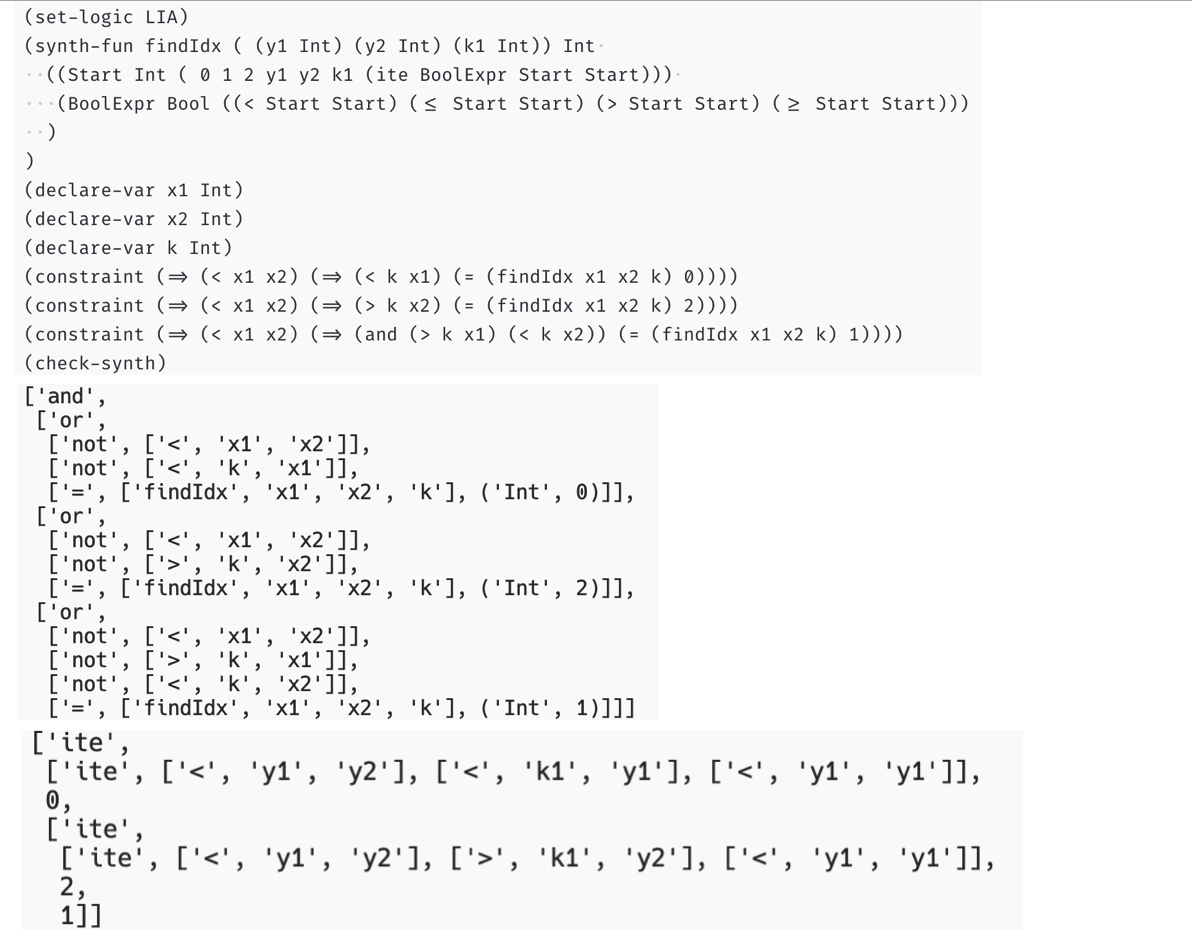
\includegraphics[width=0.8\textwidth]{example.png}
      % \caption{array\_search\_2}
    \end{figure}
  \end{frame}

  \begin{frame}
    \frametitle{效果}
    \begin{itemize}
      \item open tests中除了max和three都能解,并且可以在1s内解完。
      \item 理论上对于所有SyGuS问题,只要它对函数结果的约束只有等号约束,并且函数结果只在等号一边出现,都可以用该方法解出。
      \item \sout{并没有什么实用性。}
      \item \sout{或许可以推广到部分带有非等号约束的问题。}
    \end{itemize}
  \end{frame}

  \section{方法三:DSL增强的搜索}
  \begin{frame}
    \frametitle{动机}
    \begin{enumerate}
      \item “目前 Synthesis 方法的效率高度依赖 DSL 的设计”
      \item MaxFlash论文里和TText对比时说TText的DSL有regex所以它解的更快。
      \item 加上 $max(x,y) = ite(x<y, y, x)$这个语法糖后max问题的程序可以随便写。
    \end{enumerate}
    $\to$ 在DSL中加入一些更强的构造,并优先使用这些构造进行搜索,搜出程序后再加一个解语法糖的过程。
  \end{frame}
  \begin{frame}
    \frametitle{效果}
    max问题都可以很快的搜出来。

    我们组提交的测试用例是min15,也可以很快的搜出来。

    但我们现在只加了max和min这两个语法,只对含有需要他们的程序有优化效果。
  \end{frame}

  \section{方法四:基于Rosette的暴力展开}
  \begin{frame}
    \frametitle{算法过程}
    \begin{itemize}
      \item Rosette是Racket语言的一个扩展,提供了solver-aided programming的能力,简单来说就是可以直接把代码扔给SMT solver。
      \item 并且Rosette提供了一个$define-synthax$语法构造,可以定义一个CFG并且暴力展开k层,然后扔给SMT solver求解。
      \item 于是我们在外面套了一个对于k的迭代加深然后暴力展开求解。
      \item 实际上这个东西非常慢,不对SyGuS给出的语法做一些剪枝的话,max3都要解几分钟。
    \end{itemize}
  \end{frame}

  \section{总结}
  \begin{frame}
    \frametitle{总结}
    \begin{itemize}
      \item 我们最后的方案是并行跑直接法、DSL增强的搜索和基于Rosette的暴力展开。
      \item 实际上只需要前两种方法就可以解出open tests中的所有问题。(还带着Rosette的原因是因为时间仓促搜索法有个搜不出three的bug还没来得及修)
      \item 实现上,使用了Python, Haskell, Racket三种语言,遇到了一系列\sout{徒手造轮子}和并行问题。
    \end{itemize}
  \end{frame}

  \begin{frame}[plain]
    \addtocounter{framenumber}{-1}
    \begin{center}
      \Huge{\bf 谢谢聆听.}
    \end{center}
    \begin{figure}
      \centering
      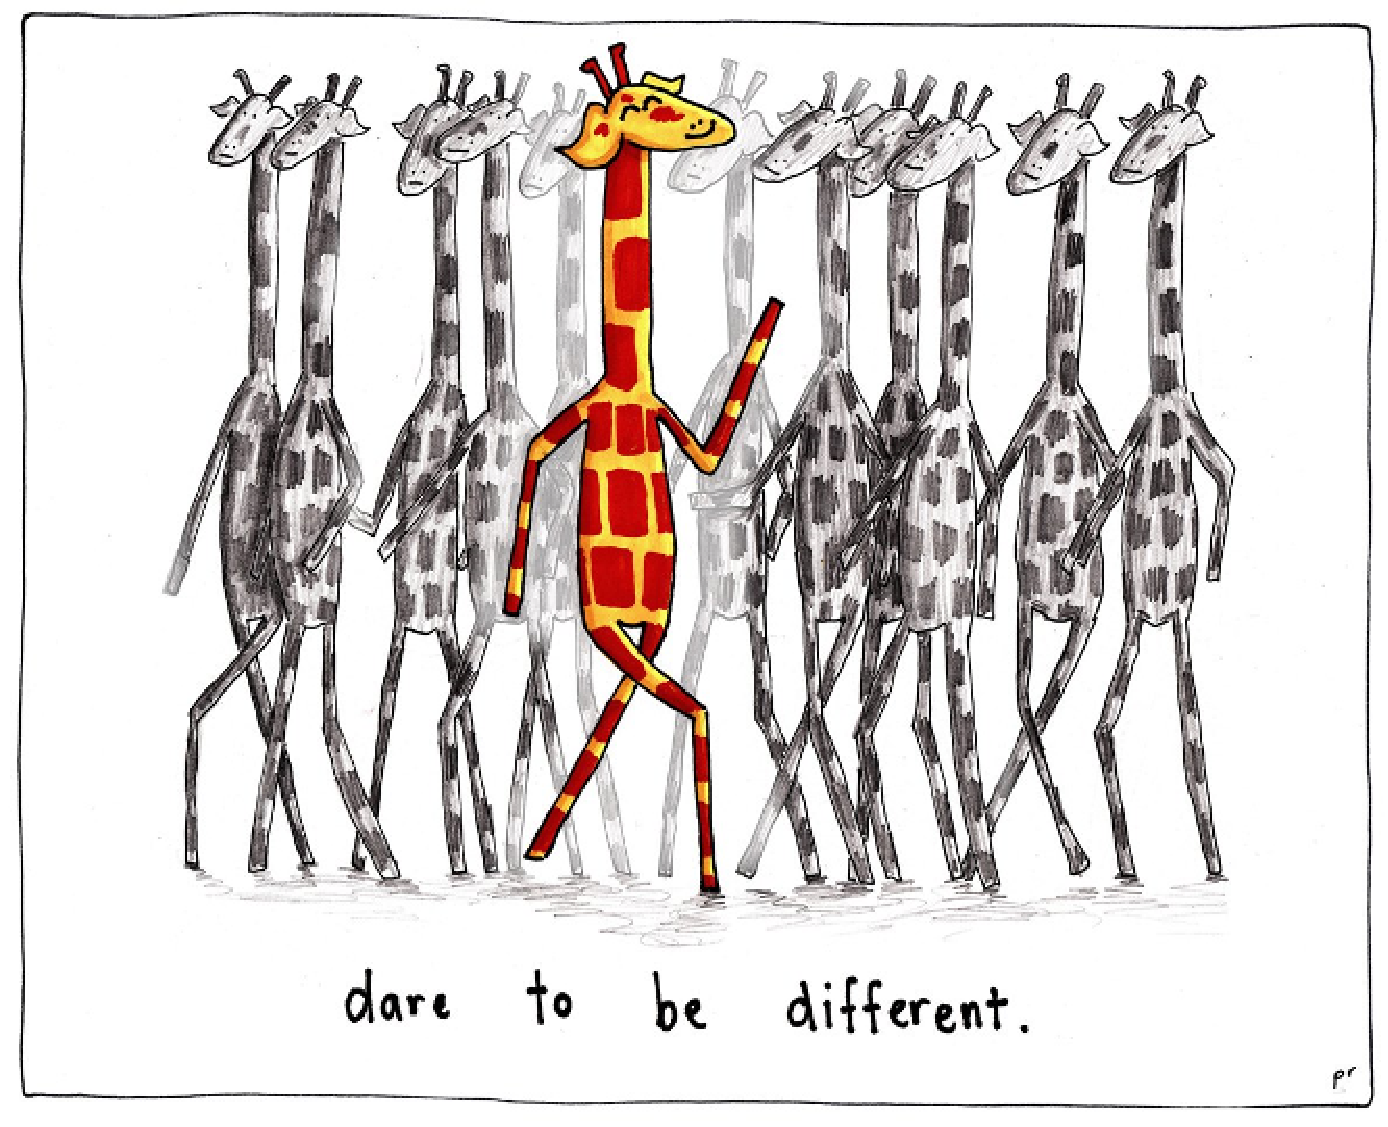
\includegraphics[width=0.5\linewidth]{dbd.pdf}
    \end{figure}
  \end{frame}
  
  
  
\end{document}